\documentclass[conference]{IEEEtran}
\IEEEoverridecommandlockouts
% The preceding line is only needed to identify funding in the first footnote. If that is unneeded, please comment it out.
%Template version as of 6/27/2024

\usepackage{cite}
\usepackage{amsmath,amssymb,amsfonts}
%\usepackage{algcompatible}
\usepackage{algorithm}
\usepackage{algorithmic}
%\usepackage{algpseudocode}
\usepackage{hyperref}
\usepackage{graphicx}
\usepackage{textcomp}
\usepackage{float}
\usepackage{xcolor}
\usepackage{booktabs}
\usepackage{lscape}
\graphicspath{{./images/}}
\def\BibTeX{{\rm B\kern-.05em{\sc i\kern-.025em b}\kern-.08em
    T\kern-.1667em\lower.7ex\hbox{E}\kern-.125emX}}
\begin{document}

\title{Game Obsession and Player engagement focused on mobile gaming enviroments\\
%{\footnotesize \textsuperscript{*}Note: Sub-titles are not captured for https://ieeexplore.ieee.org  and
%should not be used}
%\thanks{Identify applicable funding agency here. If none, delete this.}
}

\author{\IEEEauthorblockN{1\textsuperscript{st} Marshall Sharp}
\IEEEauthorblockA{\textit{Games Academy} \\
\textit{Falmouth University}\\
Falmouth, United Kindgom \\
MS279226@falmouth.ac.uk}
}

\maketitle



\begin{abstract}
In this paper, the observation of game addiction and player engagement is researched, and a test plan is created. The literature reviewed delves into the definition of Online Game Addiction (OGA) and what the effects/symptoms are, and having the debate of if it should be renamed to”Game Obsession”. The paper’s test plan also goes over the ethical, legal and professional sides of the test plan, how data from it will be handled and what risks there are with the plan, along with how to mitigate the risks.
\end{abstract}

\begin{IEEEkeywords}
engagement, obsession, mobile games
\end{IEEEkeywords}

\section{Introduction}
The nature of obsession, most notably addiction, is a difficult thing to define concisely, as we don't know for certain what classifies as an addiction in an age of technological advancements. Over the years, the definition for addiction has been made to accommodate something which, in theory, cannot apply to its original definition. It is most prevalent in the games industry, with game addiction being classified as a medical condition. This, however, could be flawed. This paper will take a look at game obsession instead of game addiction and go over game addiction and player engagement based on game obsession instead of addiction, challenging the classification of such terms.\\
\section{Background}
Gaming addiction can be defined in different ways. One paper \cite{yasir2021} defines gaming addiction with the uses and gratification theory and defines overall addiction with the medical paradigm, which has a larger emphasis on biological and psychological dependacies, which has been retrofitted to accompany the advancements of technology, and specifically in the mobile games industry. This paper also mentions that another study conducted concluded that it can be defined as the regular action of taking drastic actions in the game, such as buying in-game goods or features in a freenium game environment \cite{XWang2021}. \\

\cite{Naaj2021} was conducted during the midst of the COVID-19 pandemic in early 2020 at Ajman University, where it was found that from a sample size of 317 that have participated in an interview. They were asked three questions: \\

1) "On average, how many hours do you spend playing video games daily?"\\
This question had 17\%  of the participants who didn't play video games, though out of the participants that have, 49\% play around 2 hours on average, with 6\%  playing 8 hours and 3\% play for 10 hours. The remaining 25\%  for 5 hours as an average daily. Using this information, it can be assumed that gaming addiction affects 9\% if we're only going off of the hours one plays daily. It can be assumed based on this question alone that what causes game addiction is the amount of time played by the participant.\\

2) "Does gaming overall give you a real fulfilment in life?"\\
51\% of the 317 people interviewed said "yes", 10\% felt indifferent, and the remaining 39\% said "no".  This question contradicts question 1 of this study, as the question this poses reevaluates game addiction not based on time played but the engagement one feels for the game. The \% of people who play for 2 hours is strikingly close to how many people said "yes" to this question, so this could also be used to assume that it's about how enjoyable and engaging the game is, over how much content and play time is in the game.\\

3) "If it were needed, could you quit playing video games easily?"\\
58\% of the participating body said "yes", whilst 39\% said "no". This gives credence to the assumptions made using question 2, as over half the participants can safely withdraw from gaming entirely. However, with the quantity of participants who say they can't, it could also be assumed that it can be considered to be somewhat unreliable, as there's no proper discernable evidence to say definitively from the interview conducted.\\ 
 
4)"Did the average daily time you spend playing video games increase during [the] COVID-19 Pandemic?"\\
almost half of those who participated said "no", at 49\%. This also reinforces the assumptions made by question 2, though the volume in the "yes/no" \% is similar to question 3, with those who have said "yes" having a \% of 34. It could also be considered inconclusive.

Overall, the interview of participants states that the Average is between 2 hours and 5 hours, Most people find fulfillment in playing games, and it is just as easy to leave gaming as it is to stay, with there being no impact on people's habits over the COVID-19 Pandemic and subsequent lockdowns.\\

Naaj et al. also did ANOVA and T-tests on their hypotheses. All hypotheses revolving around these tests result in their rejection, both with a power of 0 and the same number of participants, but that is where the similarities end. Both tables in the paper revealed that more men play video games, and it does indeed affect the academic level of the students. Table one has a Lower standard deviation and higher mean for men compared to their female counterparts. This is also a similar case in table two of the paper, with females getting equal mean and deviation. This can be seen as there being little to no effect on women when it comes to gaming.\\

ANOVA tests were used to create graphs, which are figure 2 and figure 3 for this paper. Both of these factors depict a negative correlation about CGPA. It can be assumed that students who participated in this study have a higher CGPA and spend less time they spend playing video games \cite{Naaj2021}.\\

In Contrast, Rahman et al. 's \cite{Rahman2021} study focused on player engagement. The participants of this paper spent a period of 1.5 hours, up to 4+ hours on games. The most intriguing part of this paper is that even if a participant plays the bare minimum game time that was recorded in the paper, they can still consider themselves addicted to gaming. This compares to \cite{Naaj2021}, who found that the vast majority spent 2 hours playing, which fulfills \cite{Rahman2021} time period. Naaj, however, doesn't register the effects of such times played, which Rahman has reported on sleep deprivation, headaches, eye problems, eating disorders, and unhealthy mood swings. The majority of people (28.7\%) slept for 7 hours a day.\\

The effects described in \cite{Rahman2021} may affect one's health despite having no apparent effect on social health. A separate study \cite{Schlagowski2024} found that social health may not be impacted in an online format, which is in contrast to what \cite{NHSHamp24} states. From a medical standpoint, The NHS in hampshire defines gaming addiction as a variety of symptoms, with the main symptoms being reclusion from the wider world, poor hygine or lack of attention to basic needs (i.e washing, nourishments such as food or water, or sleep) and hyperfixation on gaming \cite{NHSHamp24}. \cite{Schlagowski2024} found that, despite lacking participants, a first-person view in a social simulator gets more human behaviour. The definition \cite{NHSHamp24} provides can be seen as disagreeable due to the medical paradigm being more on a biological level rather than technological. In addition, it fails to take into consideration other conditions in terms of symptoms, such as ADHD, Autism, and other neurodivergancies, which are defined in the text revision of the 5th edition of the Diagnostic and Statistical Manual of mental disorders \cite{Association2022}.\\

The concept of High Vulnerability Game Addicts and Low Vulnerability Game Addicts (HVGA and LVGA, respectively) is explored in \cite{Jing2024}'s work, utilising electroencephalography (EEG). EEG consists of technology which allows a researcher to record brain activity and normally takes the form of a headband. HVGA participants are shown to have more than their LVGA compatriots, which is something that is reflected in the results of \cite{Naaj2021}. \cite{Ruqeyya2022} paper also uses EEG, and has a minimun of 80\%  accuracy in it's results. The paper found that player engagement is vital for a mobile game to be successful, with more engagement meriting more success. This contrasts with \cite{Schlagowski2024}, which had barely any impact on player engagement for some players.

The term "Gaming Obsession" could fit this role better. One paper looks into Game Loyalty and Purchase intention \cite{Ramli2022}, in which it was found that Players who are loyal to the games they play are contradictory to a differing source they cited\cite{Widodo2020}, which has a trait of compulsive buying, which mirrors points made in \cite{yasir2021}.  This study was based on 350 out of 680 people, with the majority of the selected amount (65\%) being men and the remaining 35\% being women. The study found that from both of these groups, 55\% of the total play league for 2 -3 hours every day. The NHS  \cite{NHS2021} defines obsession as an "Unwanted or unpleasent thought, image or urge that repeatedly enters your mind, causing feelings of anxiety, disgust or unease," which is in the context of Compulsive Disorder (OCD), though it can be applied to gaming and other external areas.\\

\section{Methodology}
 The experiment will consist of two parts: An artefact which is similar to Cookie Clicker\footnote{\url{https://store.steampowered.com/app/1454400/Cookie_Clicker/}}, Utilising Unity \footnote{\url{https://unity.com/}} and stored in this repository:\\

\url{https://github.falmouth.ac.uk/MS279226/Dissertation-MS279226.git}\\

The second part of the experiment is an interview/survey form using Microsoft forms. Microsoft Forms follows GDPR practice and, due to this, is a safer form application to use when constructing this survey.

\subsection{Artefact}
The Artefact is a Unity 2023.2.20 2D project, which has a build uploaded to a phone. The game will have a "main" method of creating a point, which can be activated by tapping a large object on the screen. Gathering enough of these points will allow the participant to spend points on various autonomy methods. There will be 4 methods of autonomy that increase in price and point creation. Participants can also stack points, which adds an additive effect to both the output and the cost required to achieve the next addition to the autonomy method.\\

The UI for such a prototype may look like the following:

\begin{figure}[H]
\begin{center}
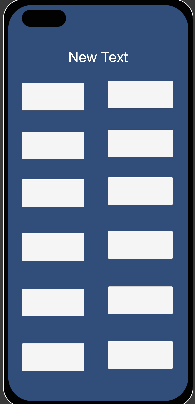
\includegraphics[width = 0.25\textwidth, ]{Sim1}
\caption{A Diagram stating how the experiment may look}
\label{tab:figure1}
\end{center}
\end{figure}

\subsection{Interview/Survey}
The second section of the experiment is an interview/survey, which will go over what the participants liked about the game, what they didn't like, and how they go about gaming habits normally. This is GDPR compliant. The survey/interview should be around 5 minutes, with a maximum of 20 minutes.

\subsection{Testing}
Unit Testing is conducted throughout the creation of the unity artefact, for integer's, floats and bools, amongst other variables.

\subsection{Recording data}
Data will be recorded in a comma-seperated Values file (.CSV). This file format makes it easier to format into graphs using programming languages such as R and Python. Utilising Python to create the graphs, Pandas, Numpy and other plugins and add-ons would need to be used. A method of data collection that could be considered is EEG, which is used in Jing's research \cite{Jing2024} and \cite{Ruqeyya2022}. However, EEG could be seen as invasive, and the institute will not have this equipment. The method chosen will be a more in-person method, manually recording the player's time played. If a participant has requested that they no longer want their data used, it will be obfuscated from the analysis and destroyed immediately after. Communication with the participant will be important as well, and contact will be kept once a month if they so request.\\

This figure (\ref{tab:figure2}) shows how the Process will go per participant:

\begin{figure}[H]
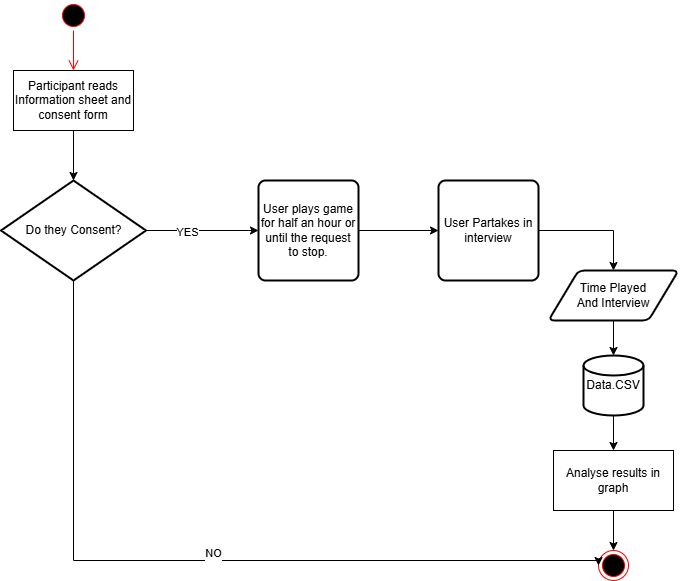
\includegraphics[width = 0.5\textwidth]{UMLProcess}
\caption{A Diagram stating how the experiment will go for a participant}
\label{tab:figure2}
\end{figure}

\subsection{Ethics and safety}
There are some things to account for with this research, to do with people and their safety. The experiment is in the hands of the participant, them being required to read an information form and sign a consent form. They can request the experiment to end early if they no longer consent to the experiment.  If they no longer consent, data will not be used when concluding and instead will be destroyed. Despite there being little physical risk, a risk assessment will still need to be carried out, with the removal of items that can be harmful for participants taking part in the research or the addition of items that can mitigate harm/ provide ease of use with the artifact.\\

\subsection{Risks}
The risks of this experiment are centered around the technology used for the experiment. As it is using a mobile device, caution must be taken if the phone is discovered to be faulty, as such faults could cause the triggering of epilepsy, burns due to the battery, and other injuries caused by the materials of the phone breaking. For this reason, the phone's hardware will be thoroughly inspected and software tested beforehand, with all faulty assets being replaced with a more stable phone. Severe software risks involve the aforementioned triggering of epilepsy, with more common risks including headaches, straining on the eyes and neck, and anxiety. For this reason, usage of software will be limited to half an hour and heavily tested. Whilst some of these scenarios are slim and may not even happen, it is better to be prepared and take measures for these edge cases.\\

Due to the paper's experiment being social and simulating obsession, it is paramount that the half an hour is upheld and is not extended, especially if the participant has any neurodivergance or is considered vulnerable. This will be mentioned as a disclaimer in the information sheet, along with a warning of epilepsy, in case any hardware/software is faulty. This time limit will also reduce the effects of screen use when interacting with the software (headaches, eye strain, etc.). \\
  
\subsection{Hypothesis}
There are two main hypotheses with this experiment, with a third one to account for the possibility of it happening:

H1: The Player will have a hyperfocus on the game and/or fulfill most of the criteria of game addiction mentioned in \cite{NHSHamp24}, though after being told it's over or requesting, they do not see a reason to keep going.\\


H2: The Player will not fulfill any criteria, so there is no change plausible.\\

H2 This is in line with Nursafika's paper \cite{Nursafika2024}, which is a study using stumble guys, a competitive party game where you compete in various minigames while being subjected to silly in-game physics. With the use of the Game Experiance Questionnaire (GEQ) method, they found that 61.46\% of participants could return to reality after playing the game, 58.30\% felt immersed in the game and 57\% felt the game had a negative affect on them, which can be see as a lesser effect when comparing that result to the 77.28\% of participants who felt the game has had a positive effect on them. At least half of all other values were above 60\%,  with the conclusion that stumble guys has little to no negative impact or addictive nature to players of stumble guys.\\

H3: The Player will fulfill the criteria of H1, but will continue with the experiment, even after it's over, either through the duration being up or from requesting it to stop. This will fulfill all of the criteria in \cite{NHSHamp24} and be classed as addiction. \\

\subsection{Questions}
There are three main questions with this research:

Q1: How long does it take for someone to consider themselves "obsessed" with the game?

Q2: Is there a correlation between perceived time playing a game and Actual time?

Q3: What truly defines addiction? Could addiction and obsession be the same?\\
\subsection{Stats testing}
Utilising G*Power, A T-test using the Point Biseral Model was conducted to determine the sample size for the experiment. Figure 3 shows that the recommended sample size using a large effect size (0.5), a 0.05 error probability and 0.8 Power will result in the sample size being 21.  With the recommended amount being about 100 participants and most sources having 200 or more, this is on the smaller end, similar to the paper Ruqeyya wrote \cite{Ruqeyya2022}, which had only 31 participants.  Python will also be used to construct the graphs for time played and compare the time played with the effect to how long, on average, the participant plays games, if any.\\

There is a Null hypothesis with the player not focusing on the game and seeing no reason to continue. This has less than 5\% chance of occuring. 

The code below is how it will be plotted:
\begin{algorithm}
\caption{The code utilised to show how the data will be plotted in python}
\begin{algorithmic}
\STATE $ graph data \gets .CSV $
\FOR {$each $ $entry$ $in$ $Data.CSV$}
	\STATE $Plot X-axis$
	\STATE $Plot Y-axis$
	\STATE $Plot Graph Points$
\ENDFOR
\STATE $printgraphtoscreen$
\end{algorithmic}
\end{algorithm}

\begin{figure}[H]
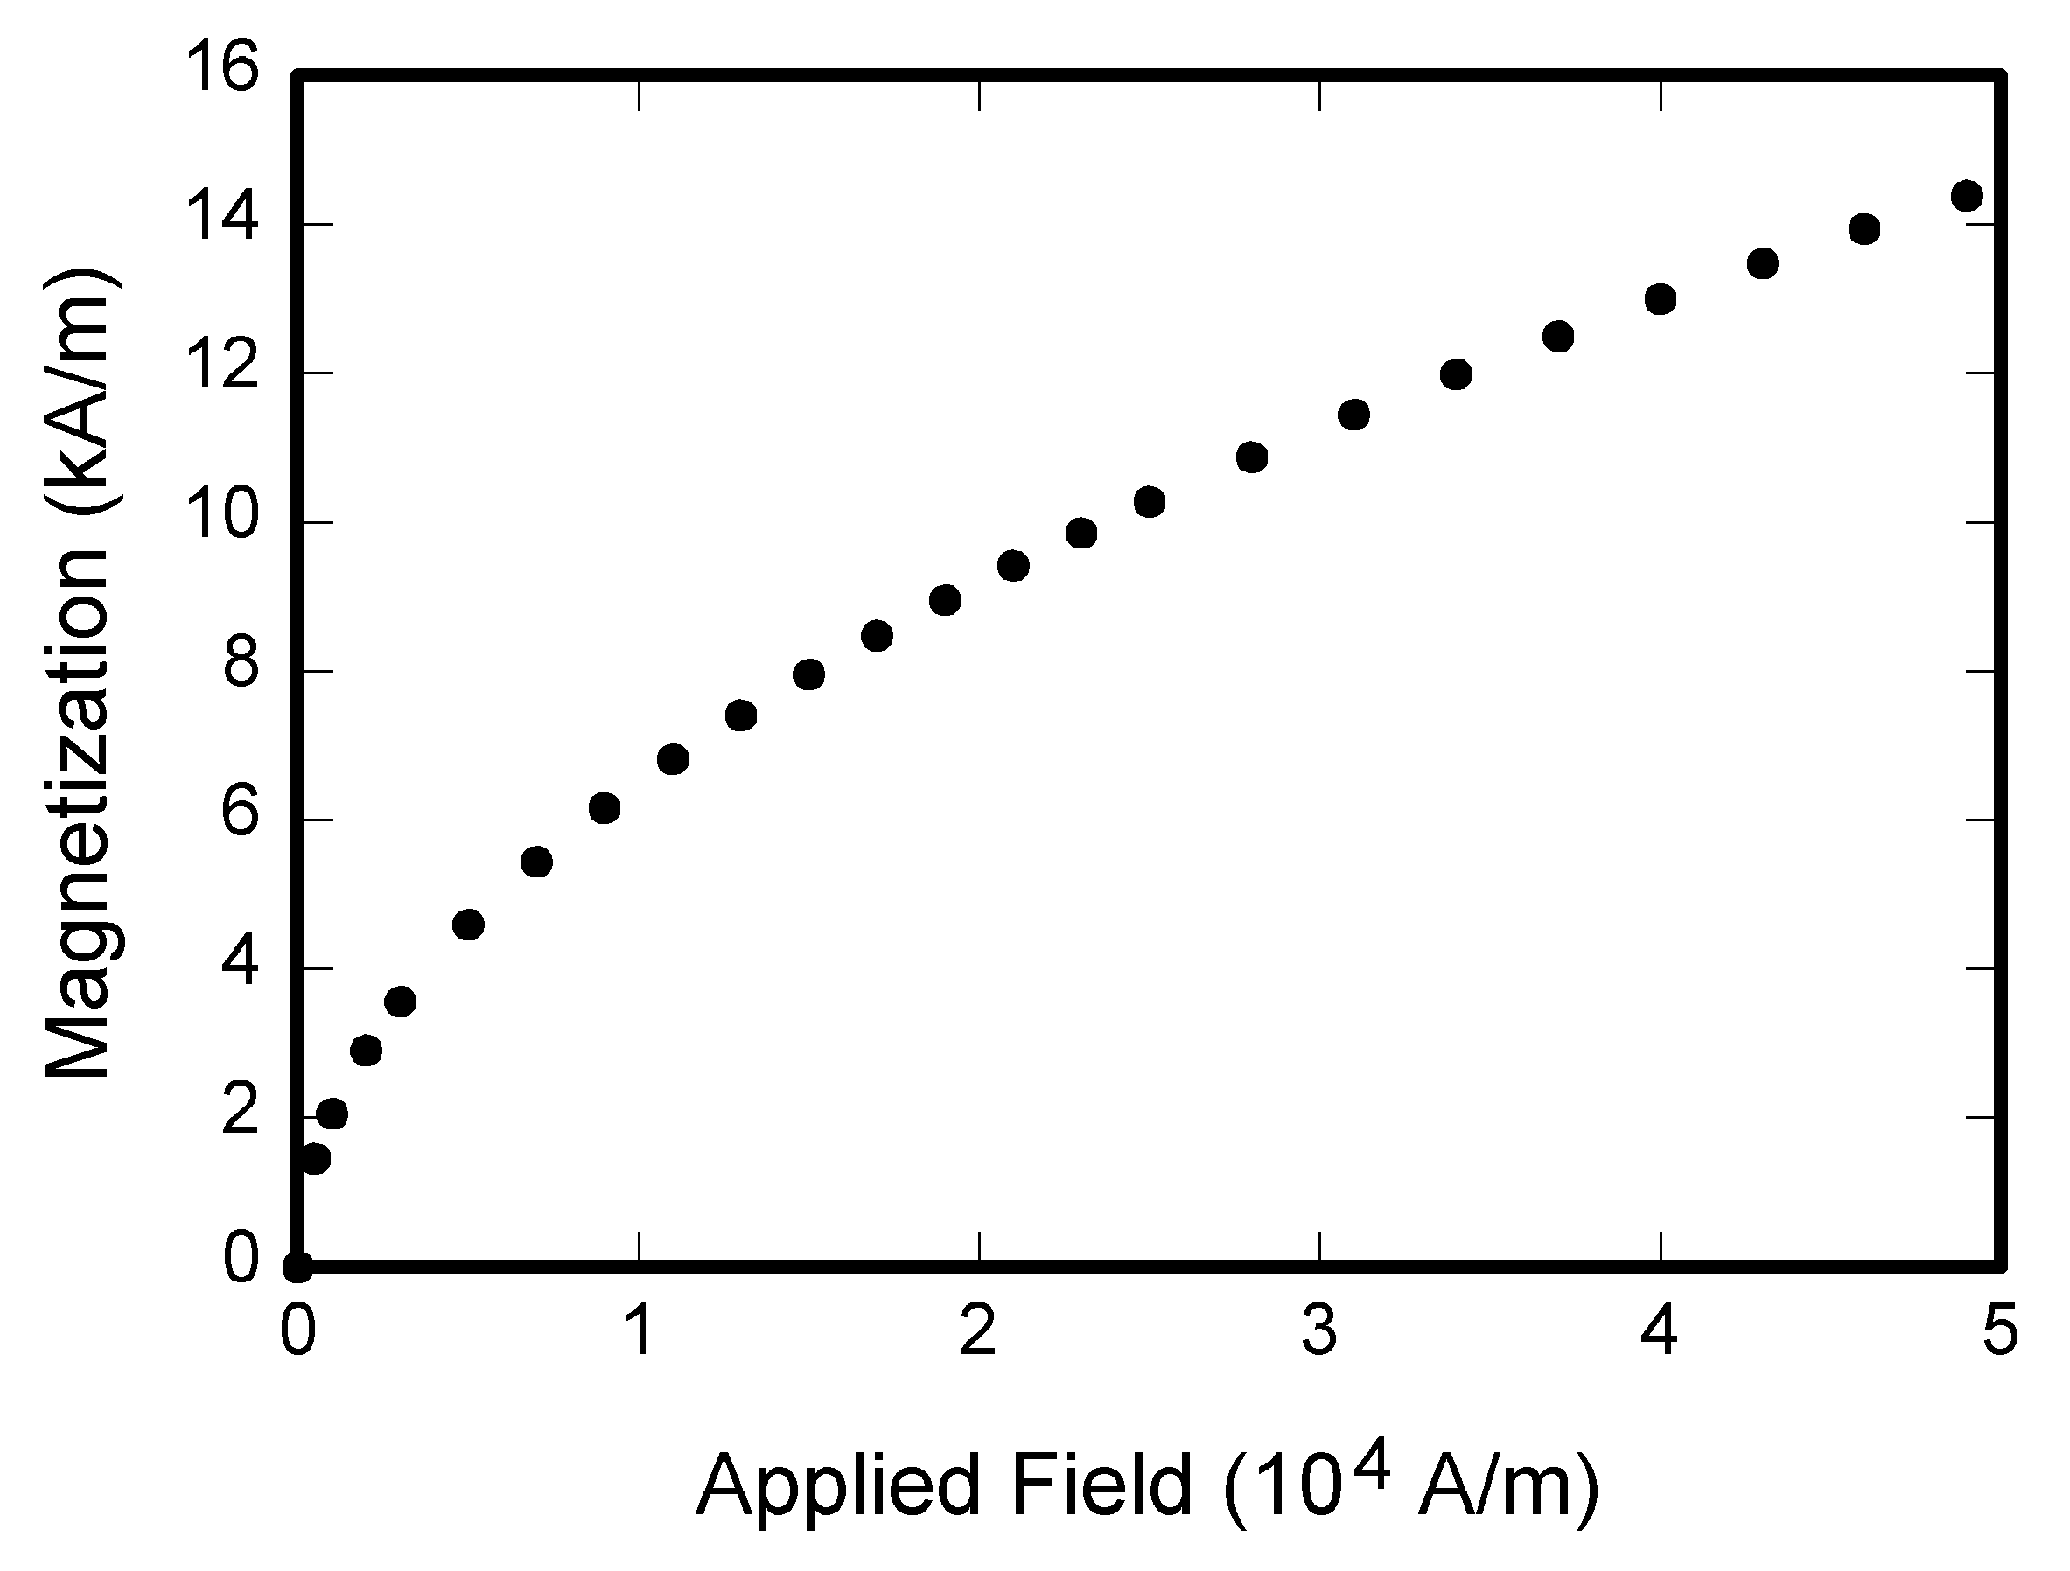
\includegraphics[width =0.5 \textwidth]{fig1}
\caption{The recommended sample size according to the G*Power t-test}
\label{tab:figure3}
\end{figure}

A Graph of the G*Power results was also plotted in the program, which portrays the increase in sample size and its correlation to the Power. This is shown in Figure 4. In addition, it can be anticipated that the sample size will more accurately be around 15 people due to the restriction of keeping the participants to the university rather than the broader public. 

\begin{figure}[H]
\includegraphics[width = 0.5\textwidth]{fig2}
\caption{The recommended sample size according to the G*Power t-test plotted as a graph, with X as the Power and Y as the sample size}
\label{tab:figure4}
\end{figure}

\subsection {Restraints}
One restraint with this research is the sample size. Due to my sample being students within the university. This limits the findings heavily, with there not being enough to get the sample size that will give a more noteworthy effect. In addition, the sample size will be limited even more due to the period for the experiment only being three weeks. This is a similar pitfall to \cite{Naaj2021} and \cite{Ruqeyya2022}.\\

\section{Results And Discussion}
\begin{table}[H]
\centering
\resizebox{0.5\textwidth}{!}{%
\begin{tabular}{@{}lll@{}}
\toprule
Participant Number & Study Time Played (minutes) & Average Time Played (minutes) \\ \midrule
1                  & 5                     & 180                           \\ \midrule
2                  & 10                    & 240                           \\
3                  & 15                    & 270                           \\
4                  & 10                    & 150                           \\
5                  & 4.2                   & 540                           \\
6                  & 5.2                   & 240                           \\
7                  & 5                     & 270                           \\
8                  & 5.4                   & 270                           \\
9                  & 5.4                   & 180                           \\
10                 & 5                     & 180                           \\
11                 & 8.6                   & 240                           \\
12                 & 5.8                   & 90                            \\
13                 & 4.3                   & 120                           \\
14                 & 15                    & 180                          
\end{tabular}%
}
\caption{Table 1 - The data collected from the experiment over two weeks.}
\label{tab:data-table}
\end{table}

After conducting the study, the results show a negative correlation. \ref{tab:data-table} shows the results plotted in the graph below \ref{tab:figure5} in conjunction with the table; the highest time recorded is 540 minutes, or 9 hours, with the average of 225
 minutes, or 3.75 hours. The average time for playing through the study came out to 6 minutes. A reason for this is due to the limitations with the study being very time-sensitive, along with the inability to find the number of participants required by my T-test. Participant 5 is a rather anomalous result due to the high amount of hours put into gaming, as mentioned in the dataset from the interview conducted alongside the artefact, whilst having the lowest recorded time within the dataset.

\begin{figure}[H]
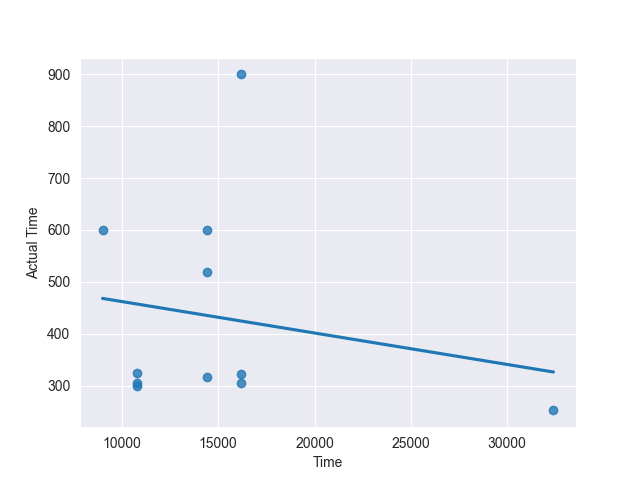
\includegraphics[width = 0.5\textwidth]{Graph1}
\caption{The correlation between perceived time and actual time.}
\label{tab:figure5}
\end{figure}

It is within reason to suspect and accept from the data that H3 is false, whilst there's plausibility that H1 is true. The best solution for clarifying this is to perform the experiment with a larger parcitipant group, along with a longer time-frame to conduct the study. H2 could also be plausible, as it is tied to the null hypothesis and will be subject to the same solution as H1.\\

From the interview, outside of asking about the hours played, some of the questions include:\\

A) When you hear of game addiction, what does your mind immediately think of?\\

This question spurred many answers of what the perception of OGA, with the majority of answers having things in common. The perception of OGA follows Reclusion, prolonged behaviour that is detrimental both to ones health and finances and with that prolonged behaviour, difficulty functioning in society. Though other answers exemplify a specific game titles, like World of Warcraft, league of legends and final fantasy 14, which are known to have massive player-bases over the years they have be avalible. Some answers express a generational divide, such as one answer claiming defamatory news articles written by an out-of-touch older generation or grandparents telling them one hour is way too long for a session of video games.\\

One answer out of the Fourteen is an interesting teake on the topic: "Just like hobbies, people tend to misinterpret a video game hobby. They claim it's addiction but it's just a usual thing you love doing." harkens at the fact someone might love what they do with their hobbies to be societally seen as addicted. This answer for this question, whilst opinionated, does show that whilst most people have some form of negative outlook on what OGA is, it could also be argued that, to a lesser extent, is simply the overbearing love for what they enjoy when not dealing with the mundanity of life.\\

B) - The definition of addiction the NHS uses revolves around the use of substances, with it's definition being defined as \textbf{"not having control over doing, taking or using something to the point where it could be harmful to you"}. Using this definition, does it accurately fit your relation to gaming?\\

12 ( or 86\%) of the participants answered this question with "no", whilst only 2 (or 14\%) affirmed this definition to their relation with gaming. When asked why, most responses followed a structure of self control and moderation, though once again highly opinionated. Most answers normally consist of "because I do/have X (where X is a habit used to moderate their time playing video games), I do not belive I suffer from it(OGA).". Interesting answers come from those that affirmed, with "I do stop playing when needed to...When  the game gets good I keep trying to play "one more game"." and "My state with games is using them to keep a healthy state of mind; the issue I have is making sure gaming and gaming-related activited do not become one."\\

The general consensus from this question is mainly you have ways of moderating it, even if creating that moderation seems difficult.\\

C) Do you think "Game Obsession" would be better suited as a name for game addiction? why?
The Majority of the answers for the question reflect a negatory response, mainly refering to it as a "gateway term", and that addiction is still an ongoing issue. 


\section{Conclusion}


\bibliographystyle{IEEEtran}
\bibliography{Dissertationbib.bib}

\end{document}
